\documentclass[class=article, crop=false]{standalone}
\usepackage[subpreambles=true]{standalone}
\usepackage{import}
\usepackage[T1]{fontenc}
\usepackage[utf8]{inputenc}
\usepackage[english, danish]{babel}
\usepackage{graphicx,wrapfig,lipsum}

\begin{document}
    Et aktivitetsdiagrammer er på Figur~\ref{fig:activity_diagram}
    lavet for at få et overblik over hvordan vores overordnede matador-program skal køres, altså uden yderligere aktivitetsdiagrammer over det de mindre funktionaliteter såsom “Administrer grunde” og “Køb grund”, som der kun refereres til. Figur~\ref{fig:activity_diagram} kan bruges igennem hele projektet som reference til, hvordan spillet skal forløbe, og hvad de overordnede regler er.\par
    Senere blev der også tildelt farver for at have en visuel repræsentation af hvor langt projektet er kommet. Rød for ikke implementeret, gul for delvist implementeret og grøn for fungerende implementation.


    \begin{figure}[H]

        \hbox{\hspace{-3cm} 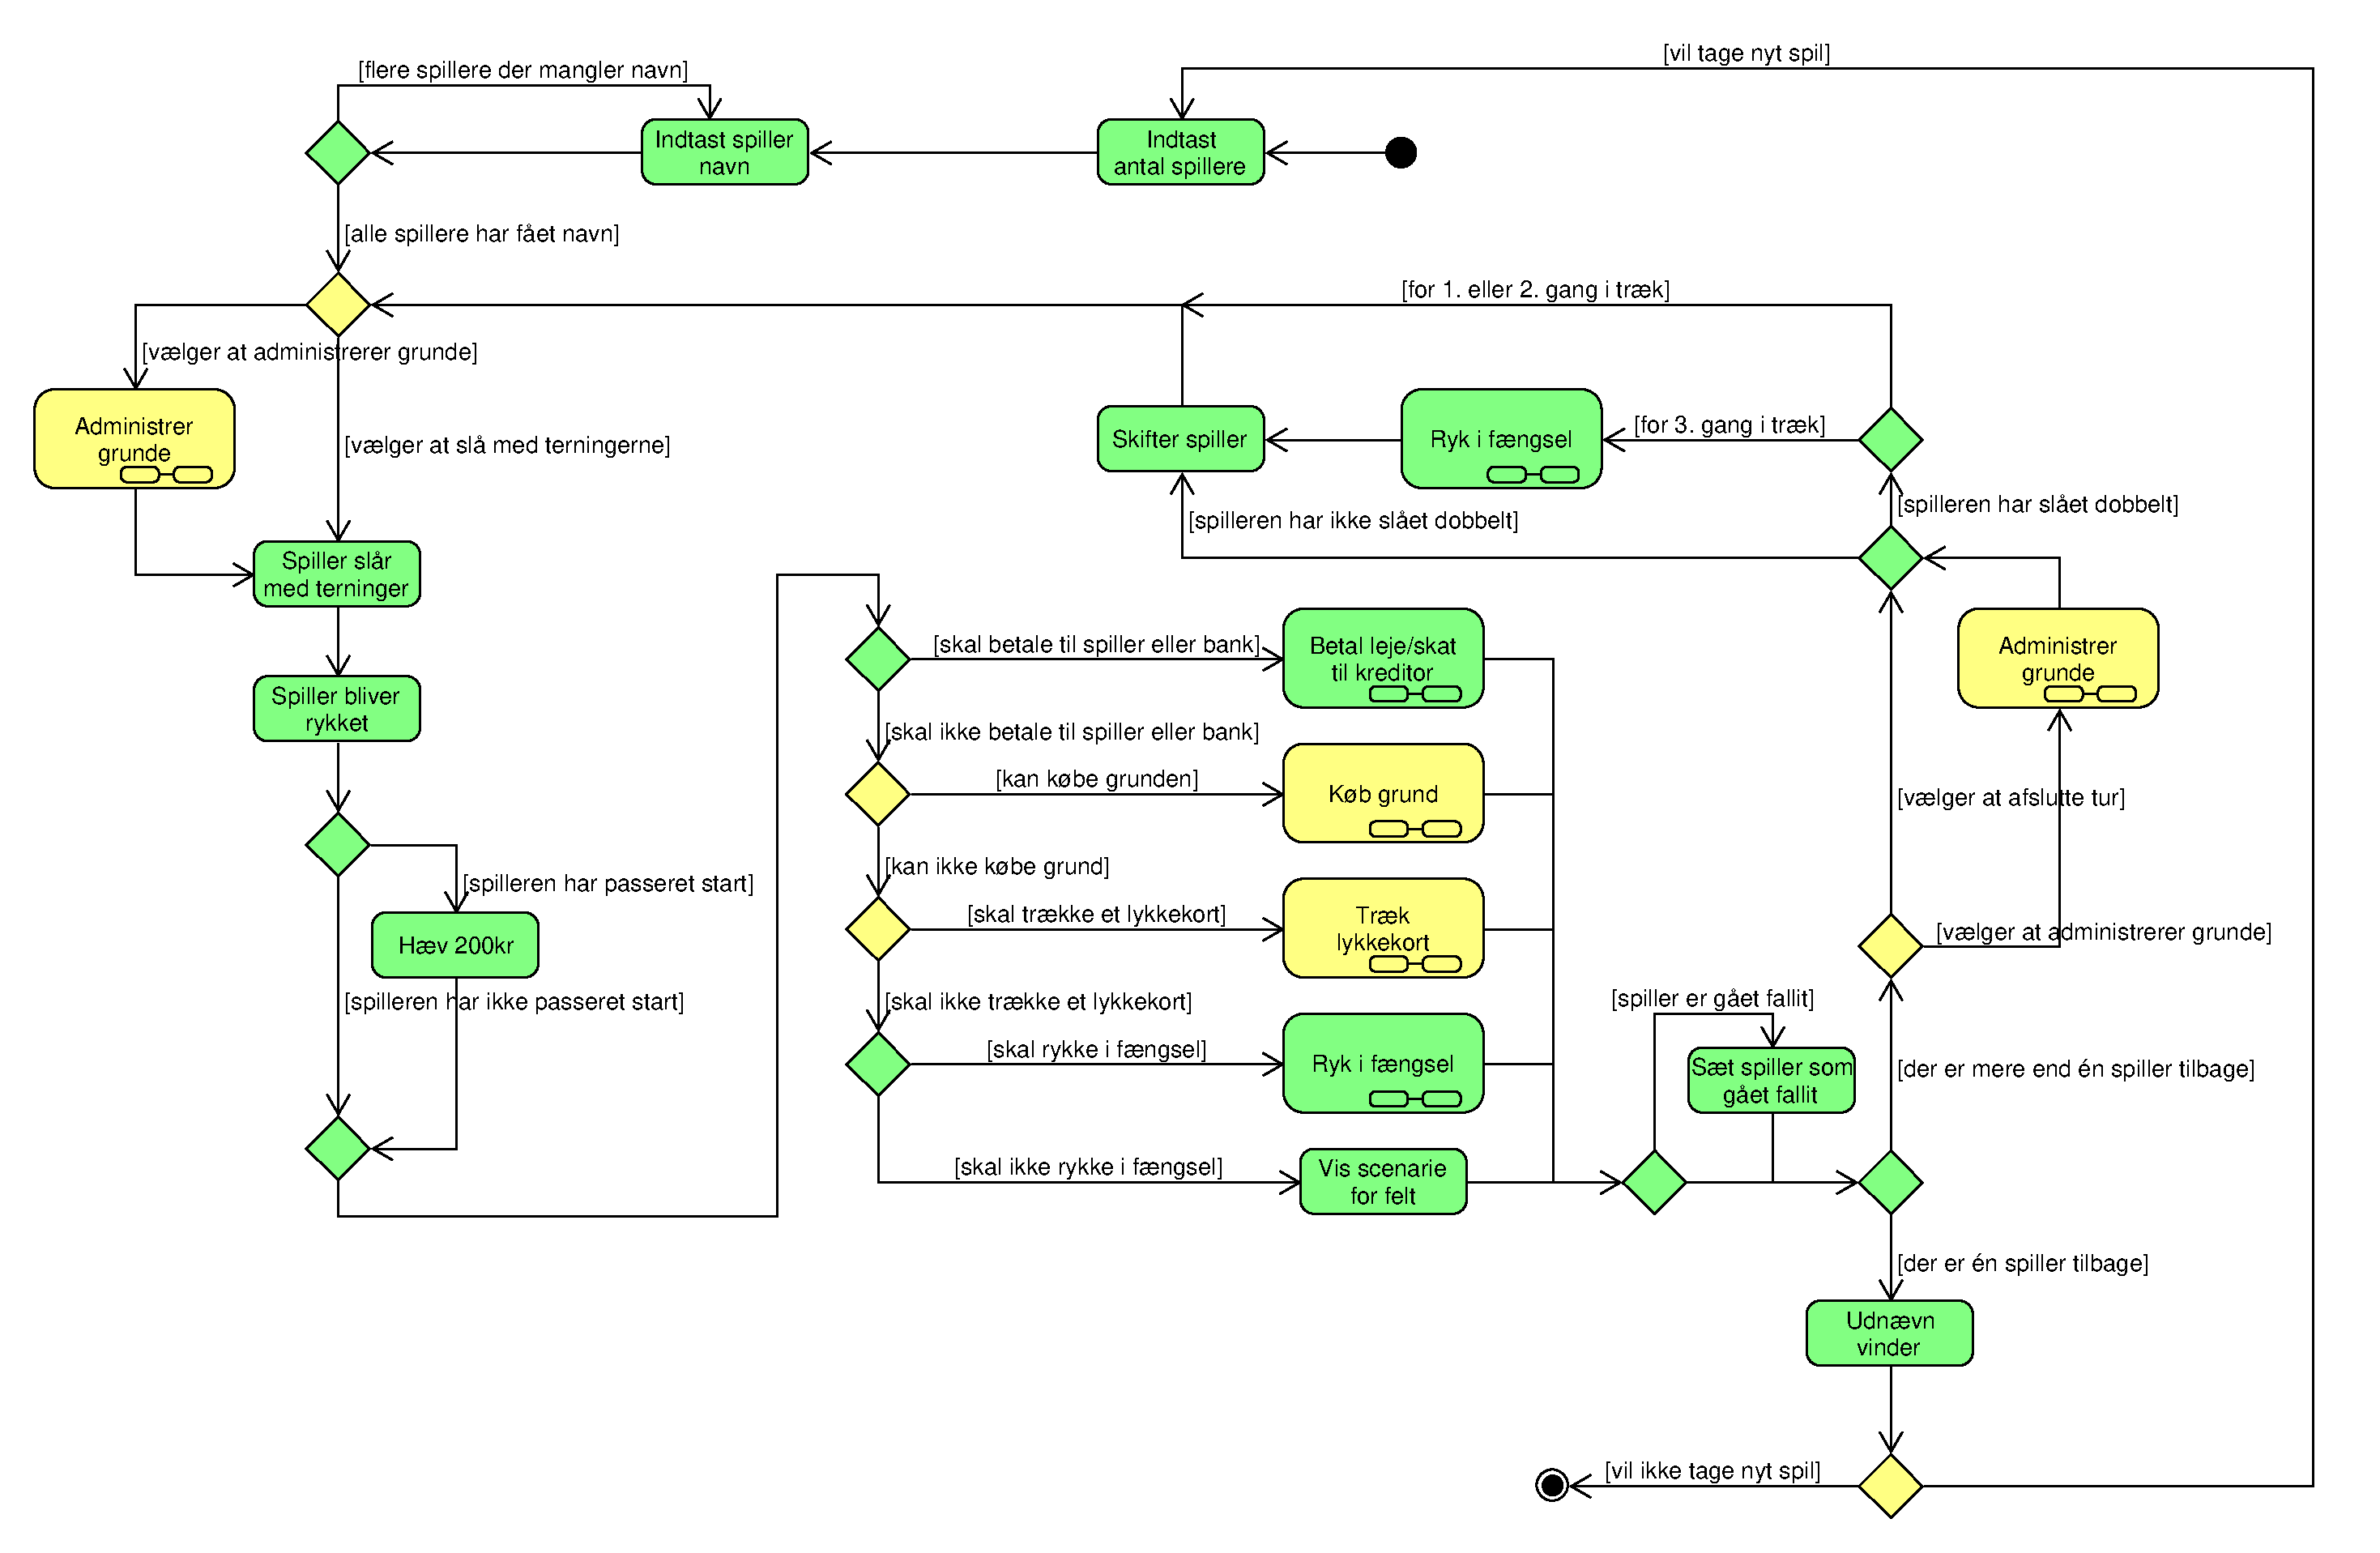
\includegraphics[scale=0.455]{diagrams/activity_diagram.pdf}}

        \caption{Domænemodellen over systemet}\label{fig:activity_diagram}
    \end{figure}

\end{document}